\chapter{Detalles de Implementación de \maggen}
\label{chap:implem}
\minitoc

En esta sección se aclararan y expondrán decisiones que se realizaron a lo largo de la implementación de esta herramienta.

Primero, como ya se menciona en el capítulo anterior, el lenguaje sobre el cual se realizó el desarrollo de \maggen\ es C++, con lo que todo el código es principalmente característico de un modelo de ``Programación Orientado a Objetos'', aunque posee secciones de ``Programación Imperativa'', para lograr optimizaciones y poder integrar componentes externos.

\section{Parsing usando \boost\ \spirit}
\label{sec:par-spirit}
El primer desafío de codificación, fue parsear el archivo de entrada de la herramienta, en el cual vendría la especificación de una Gramática de Atributos. Dicho parser debía respetar las condiciones ya analizadas en el capítulo anterior (Ver sección \ref{sec:lenguajeMAG}). 

La solución obtenida se apoya en la utilización de un framework reconocido mundialmente, denominado \spirit, perteneciente a la biblioteca de C++ llamada \boost. Esta decisión trajo dos grandes beneficios; la confiabilidad del parser obtenido y la rápida obtención del mismo, ya que, la gran ventaja de \spirit es permitir escribir la definición de la gramática en lenguaje \textbf{C++}.

\spirit\ es un framework generador de analizadores sintácticos, o parsers, descendentes recursivos orientado a objetos implementado usando técnicas de meta-programación con plantillas. Las expresiones mediante plantillas, permiten aproximar la sintaxis de una ``\textit{\textit{Forma Backus Normal Extendida}}'' (\textbf{EBNF}) completamente en C++.

\spirit es un producto en continua evolución y desarrollo; actualmente se encuentra en la versión $2.3$. A partir de la $2.0$, se integraron todas los componentes anteriores dentro de ``\spirit.\textit{Classic}''. Demás componentes son encapsulados en dos nuevas capas\footnote{Detalles sobre las mismas pueden ser encontradas en\\ \urllink{http://www.boost.org/doc/libs/1\_43\_0/libs/spirit/doc/html/index.html}}: \textit{Qi} y \textit{Karma}. Para el desarrollo del parser de \maggen\ se utilizaron componentes propios de \spirit.\textit{Classic}, por cuestiones de simplicidad y compatibilidad. 

Se puede resumir el proceso de análisis sintáctico, en este framework, en cuatro componentes, como lo muestra la figura \ref{fig:procesoSpirit}.

\begin{figure}[!ht]\centering
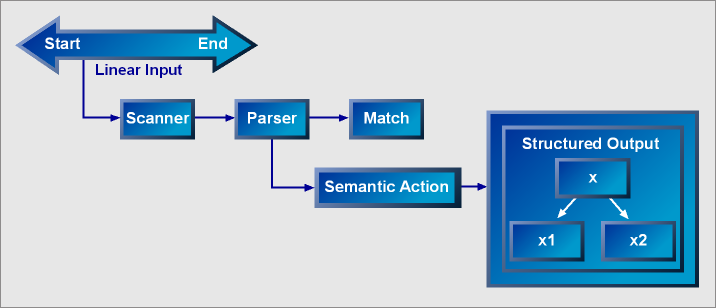
\includegraphics[width=400pt, height=160pt]{./spirit.png}
\caption{Procesos dentro de \spirit}\label{fig:procesoSpirit}
\end{figure}

El usuario es el responsable de definir las ``\textbtt{semantic actions}'' para lograr capturar los resultados intermedios, producidos durante la etapa de parsing y no sólo obtener un valor lógico, sobre si se pudo o no consumir toda la cadena de entrada.

Para comenzar a definir una gramática hay que crear una estructura que herede de la clase \textbtt{grammar}. Dentro de ella se debe definir a su vez otra estructura templatizada denominada \textbtt{definition}. En donde realmente estará la definición de la gramática.

Para definirla, se dispone de un amplio conjunto de herramientas. Primero, los operadores de metalenguaje listados en la tabla \ref{ope_spirit}, los cuales permiten construir nuevas reglas combinando reglas ya definidas, parsers y constantes permitidas en el framework.

\begin{table}[!ht]\centering
\begin{tabular}{| c | l |}
\hline

\rowcolor{gris} \textbf{Operador} & \textbf{Semántica} \\ \hline

A $=$                  B  & Definición de A en base a B \\ \hline
A $|$                  B  & Unión, acepta A o B, también llamada ``alternativa''\\ \hline
A $\&$                 B  & Intersección, acepta A y B \\ \hline
A $-$                  B  & Diferencia, acepta A pero no a B  \\ \hline
A \textasciicircum     B  & Disyunción exclusiva, acepta A o B, pero no a ambos \\ \hline
A $>>$                 B  & Secuencia, acepta A seguido de B \\ \hline
\multirow{2}{*}{A $\%$ B} & Lista, acepta A separados por ocurrencias de B.\\
                          & Es equivalente a: A $>>$ *(B $>>$ A)\\ \hline
$*$                    A  & Estrella de Kleene, 0 o más veces \\ \hline
$+$                    A  & Positivo, 1 o más veces \\ \hline
$!$                    A  & Opcional, 0 o 1 vez \\ \hline
\end{tabular}
\caption{Operadores de \spirit\ utilizados}\label{ope_spirit}
\end{table}

Por otra parte, \spirit\ dispone de un gran conjunto de parsers que abarcan la mayoría de los tipos básicos, representación de datos y valores utilizados en el común de los lenguajes (ver tabla \ref{parsers}).

\begin{table}[!ht]\centering
\begin{tabular}{| l | l |}
\hline

\rowcolor{gris} \textbf{Parser} & \textbf{Entrada aceptada} \\ \hline

anychar\_p & Cualquier carácter simple (incluyendo el carácter nulo: '$\setminus0$')\\ \hline
alnum\_p   & Caracteres alfa-numéricos \\ \hline
alpha\_p   & Caracteres alfabéticos \\ \hline
% blank\_p & Un espacio o tabulación \\ \hline
digit\_p   & Dígitos numéricos \\ \hline
lower\_p   & Caracteres en minúscula \\ \hline
upper\_p   & Caracteres en mayúscula \\ \hline
space\_p   & Espacios, tabulaciones, saltos de línea y nuevas líneas \\ \hline
ch\_p      & Carácter especificado como parámetro \\ \hline
str\_p     & Cadena especificada como parámetro \\ \hline
oct\_p     & Dígito en octal \\ \hline
hex\_p     & Dígito en hexadecimal \\ \hline
uint\_p    & Número entero sin signo de 32 bits \\ \hline
int\_p     & Número entero 32 bits \\ \hline
real\_p    & Número flotante 32 bits \\ \hline
eps\_p     & Cadena vacía (épsilon) \\ \hline
end\_p     & Carácter de fin de archivo (\textbtt{EOF}) \\ \hline
\end{tabular}
\caption{\label{parsers} Parsers predefinidos de \spirit\ utilizados} 
\end{table}

Además posee varias directivas que modifican el comportamiento de los parsers, encapsulándose en una expresión definida por el usuario (ver tabla \ref{directivas}).

\begin{table}[!ht]\centering
\begin{tabular}{| l | l |}
\hline

\rowcolor{gris} \textbf{Directiva} & \textbf{Efecto} \\ \hline

lexeme\_d    & Deshabilita la omisión de espacios en blanco (\textbtt{space\_p})\\ \hline
as\_lower\_d & Convierte en minúscula lo aceptado por la expresión\\ \hline
\multirow{3}{*}{longest\_d} & Deshabilita el corto circuito, manda al analizador que\\
                            & pruebe todas las alternativas posibles y elija la secuen-\\
                            & cia más larga aceptada \\ \hline
\end{tabular}
\caption{\label{directivas} Directivas de \spirit\ aplicadas}
\end{table}

El prototipo para la gramática es el siguiente:

\begin{lstlisting}[float=!ht, columns=fullflexible, linewidth=9cm]
struct my_grammar: public grammar <my_grammar>
{
    template <typename ScannerT>
    struct definition
    {
        rule <ScannerT> r;

        definition(my_grammar const& self)
        {
            r = /*... Aqui va la definicion ...*/;
        }
        rule <ScannerT> const& start() const
        {
            return r;
        }
    };
};
\end{lstlisting}

Para el manejo de los símbolos válidos dentro de la definición de la gramática, \spirit\ soporta nativamente, el concepto de ``Tablas de símbolos''. Lo que permite registrar de manera dinámica nuevos símbolos, en particular dentro de la herramienta permitió manejar los conjuntos de nombres válidos para los \textbtt{sorts}, los símbolos no terminales permitidos en las ecuaciones, entre otros usos.

Para comenzar a interactuar con el framework, el usuario debe declarar un objeto de la estructura definida y pasarlo como parámetro a una función específica de \spirit.

\begin{lstlisting}[float=!ht, columns=fullflexible, linewidth=7cm]
my_grammar g;

if (parse(first, last, g, space_p).full)
{
  cout << "Parsing Succeeded\n";
}
else
{
  cout << "Parsing Failed\n";
}
\end{lstlisting}


\section{Gramática de Atributos con \spirit}
\label{sec:gramspirit}
Lo primero que se tuvo que realizar, fue definir los componentes básicos que se iban a necesitar para construir las demás declaraciones.

\begin{description}
\item [Identificadores] son los nombres de sorts, funciones, atributos, símbolos no terminales y reglas, permitidos por \maggen\ y se definen como en el común de los lenguajes. Debido a que el lenguaje del evaluador generado es C++, todas las palabras reservadas de ese lenguaje, son de la misma clase para \maggen.

\begin{lstlisting}[float=!ht, columns=fullflexible, linewidth=12.6cm]
r_ident = lexeme_d[(alpha_p|'_')>>*(alnum_p|'_')]-r_reserved_word;

r_reserved_word = str_p("compute")|"end"
                              | "all"
                              | "semantic domain"|"attributes" |"rules"
                              | "sort"|"op"|"function"
                              | "infix"|"prefix"|"postfix"
                              | "syn"|"inh"
                              | "left"|"right"|"non_assoc"
                              | r_cpp_reserved_words;

r_cpp_reserved_words = r_cpp_basic_types
                                       | str_p("and")|"and_eq"|"asm"|"auto"|"bitand"
                                       | "bitor"|"break"|"case"|"catch"|"class"|"compl"
                                       | "const"|"const_cast"|"continue"|"default"
                                       | "delete"|"do"|"double"|"dynamic_cast"|"else"
                                       | "enum"|"explicit"|"export"|"extern"|"false"
                                       | "for"|"friend"|"goto"|"if"|"inline"|"long"
                                       | "mutable"|"namespace"|"new"|"not"|"not_eq"
                                       | "operator"|"or"|"or_eq"|"private"|"protected"
                                       | "public"|"register"|"reinterpret_cast"|"return"
                                       | "short"|"signed"|"sizeof"|"static"|"static_cast"
                                       | "struct"|"switch"|"template"|"this"|"throw"|"true"
                                       | "try"|"typedef"|"typeid"|"typename"|"union"
                                       | "unsigned"|"using"|"virtual"|"void"|"volatile"
                                       | "wchar_t"|"while"|"xor"|"xor_eq";

r_cpp_basic_types = str_p("bool")|"char"|"float"|"int"|"string";
\end{lstlisting}

\item [Operadores] Dentro de la especificación de la GA, se permiten como nombre válidos para los operadores, caracteres alfabéticos, numéricos y los operadores básicos de C++. 

\begin{lstlisting}[columns=fullflexible, linewidth=11.5cm]
r_oper = lexeme_d[(alpha_p|'_'|r_id_op)>>*(alnum_p|'_'|r_id_op)];

r_id_op = ch_p('+')|'*'|'/'|'^'|'%'|'&'|'<'|'='|'-'|'>'|'|'|'~'|'.'|', '|'?';
\end{lstlisting}

\item [Literales] Son los valores de constantes y tipos básicos aceptados, se adecuan a los estándares de C++. Solamente se tuvo que definir los valores lógicos, los caracteres entre comillas simples y las cadenas de caracteres entre comillas dobles, ya que para los tipos numéricos, existen parsers predefinidos de \spirit\ como ya se dio a conocer.

\begin{lstlisting}[columns=fullflexible, linewidth=10.7cm]
r_boolean = str_p("true")|"false";

r_char = lexeme_d[ch_p('\'')>>(anychar_p)n>ch_p('\'')];

r_string = lexeme_d[ch_p('\"')>>r_string_lit>>ch_p('\"')];

r_string_lit = +((anychar_p-(ch_p('\"')|"\\"|'\'' ))|r_esc_seq);

r_esc_seq = ch_p('\\')>>
                  ( oct_p
                  | as_lower_d['x']>>hex_p
                  | (anychar_p-ch_p('\n'))
                  );
\end{lstlisting}
\end{description}

Para tener una consistencia de identificadores para cada componente de la gramática, se utilizaron \textit{tablas de símbolos} como repositorio. Además, gracias a que \spirit, también se utilizaron como reglas dinámicas, limitando posibles valores en definiciones que las incorporaran.

\begin{lstlisting}[columns=fullflexible, linewidth=5.5cm]
symbols <> st_sorts;
symbols <> st_op_prefix;
symbols <> st_op_infix;
symbols <> st_op_postfix;
symbols <> st_functions;
symbols <> st_attributes;
symbols <> st_non_terminal;
\end{lstlisting}

\subsection{\textbtt{``semantic domain''} en \spirit}

En esta sección de la especificación se debían aceptar tres tipos de elementos: \textbtt{sorts}, \textbtt{operators} y \textbtt{functions}.

Los \textbtt{sorts} serán los tipos que se podrán utilizar para definir los dominios e imágenes de los operadores y funciones.

Teniendo en cuenta lo analizado en la sección \ref{subsec:bloq-sem}, a continuación se analizan algunas consideraciones de implementación.

\begin{description}
\item [\textbtt{sorts}] Se exige que luego del identificador ``\textbtt{sort}'' existe un espacio\footnote{\label{foot:espacio}Ver definición de \textbtt{space\_p} en \ref{parsers}}. El nombre leído, se usará para crear un nuevo Sort dentro de la GA y también se insertará en la tabla de símbolos de sorts. Se acepta una lista de nombres de sorts para comodidad del usuario.

\begin{lstlisting}[columns=fullflexible, linewidth=11cm]
r_decl_sort = lexeme_d[str_p("sort")>>space_p]>>
                        (r_ident[&create_sort][st_sorts.add]%', ')>>';';
\end{lstlisting}

\item [\textbtt{operators}] Para los operadores también se exige el espacio$^{\ref{foot:espacio}}$ luego de la cadena ``\textbtt{op}''. Por definición se aceptan tres tipos: infijos, prefijos y posfijos, por lo que se hizo una regla para cada uno, solamente discriminado los dominios, ya que todos poseen una sóla imagen. Notar que los sorts permitidos, son sacados directamente de las tablas de símbolos destinadas para ese propósito.

\begin{lstlisting}[columns=fullflexible, linewidth=12.5cm]
r_decl_oper = lexeme_d[str_p("op")>>space_p][&inic_func]>>
                        (r_oper_infix|r_oper_postfix|r_oper_prefix)>>
                        str_p("->")>>
                        r_sort_st[&save_image_func]>>';';

r_oper_infix = str_p("infix")[&save_mode_op]>>
                          !r_oper_mode>>
                          r_oper[&save_name_func][st_op_infix.add]>>':'>>
                          r_sort_st[&save_domain_func]>>', '>>
                          r_sort_st[&save_domain_func];

r_oper_postfix = str_p("postfix")[&save_mode_op]>>
                              !r_oper_mode>>
                              r_oper[&save_name_func][st_op_postfix.add]>>':'>>
                              r_sort_st[&save_domain_func];

r_oper_prefix = !(str_p("prefix")[&save_mode_op])>>
                            !r_oper_mode>>
                            r_oper[&save_name_func][st_op_prefix.add]>>':'>>
                            r_sort_st[&save_domain_func];

r_oper_mode = '('>>
                         (uint_p[&save_prec_op]|'_')>>', '>>
                         (r_oper_assoc[&save_assoc_op]|'_')>>
                         ')';

r_oper_assoc = str_p("left")|"right"|"non_assoc";
\end{lstlisting}

\item [\textbtt{functions}] Para las funciones se permiten como dominio listas de sorts, los cuales serán agregados incrementalmente a la función que se está declarando. La utilización de acciones semánticas facilitan la modularización. La declaración comienza con la cadena ``\textbtt{function}'' seguida de una espacio$^{\ref{foot:espacio}}$.

\begin{lstlisting}[columns=fullflexible, linewidth=12.7cm]
r_decl_func = lexeme_d[str_p("function")>>space_p]>>
                        r_oper[&inic_func][&save_name_func][st_functions.add]>>
                        ':'>>
                        !r_dom_func>>
                        str_p("->")>>
                        r_sort_st[&save_image_func]>>
                        ';';

r_dom_func = r_sort_st[&save_domain_func]%', ';
\end{lstlisting}
\end{description}

\subsection{\textbtt{``attributes''} en \spirit }

Para la codificación de esta sección la funcionalidad buscada era que el usuario mediante una expresión en términos de conjuntos definiera la pertenencia de cada atributo. Por lo que se tuvo que implementar un ``mini-intérprete'' sobre expresiones de conjuntos.

Un detalle a tener en cuenta, en este punto, es que no se encuentra declarado ningún símbolo no terminal'', así que todo símbolo mencionado dentro de la expresión será creado bajo demanda.

La vinculación de los atributos con sus respectivos dueños, se realizará más adelante, debido a que existe la posibilidad de declarar un atributo para todo símbolo, mediante la sentencia \textbtt{all}, antes de tener totalmente definido el conjunto de símbolos no terminales de la gramática.

\begin{lstlisting}[columns=fullflexible, linewidth=12cm]
r_attributes = lexeme_d[str_p("attributes")>>space_p]>>
                          +r_decl_attr[&create_attributes];

r_decl_attr = (r_ident[&add_attribute][st_attributes.add]%', ')>>
                         ':'>>
                         !(r_type_attr[&save_type_attr])>>
                         '<'>>r_sort_st[&save_sort_attr]>>'>'>>
                         lexeme_d[str_p("of")>>space_p]>>
                         (r_conj_symb |
                         (str_p("all")n>!('-'>>r_conj_symb))
                         )[&save_member_list_attr]>>
                         ';';

r_conj_symb = '{'>>(r_ident%', ')>>'}';

r_type_attr = str_p("inh")|"syn";
\end{lstlisting}

\subsection{\textbtt{``rules''} en \spirit}

En la definición de una gramática las reglas son los pilares, por eso en esta sección se debía brindar la mayor flexibilidad al usuario.

El bloque de reglas comienza con el identificador ``\textbtt{rules}'', seguida de un espacio$^{\ref{foot:espacio}}$ y una lista de reglas. Cada una de las mismas son enumeradas desde 1 para mantener una indexación interna. Una vez consumido el bloque se realizan los chequeos que determinan si la GA es MAG o no\footnote{Detalle sobre MAG, ver capítulo \ref{chap:mag}.}.

\begin{lstlisting}[columns=fullflexible, linewidth=10cm]
r_rules = lexeme_d[str_p("rules")>>space_p]>>
                 (+r_decl_rule)>>eps_p[&check_well_defined];
\end{lstlisting}

Una regla individualmente esta representada por un identificador y los caracteres ``\textbtt{::=}'' y una lista de símbolos, dejando también la posibilidad de escribir reglas abreviadas mediante el uso del operador ``|'' junto a una nueva lista de símbolos, evitando repetir el lado izquierdo de la regla.

\begin{lstlisting}[columns=fullflexible]
r_decl_rule = r_ident[&create_new_non_terminal][&create_rule][st_non_terminal.add]>>
                        str_p("::=")>>
                        r_right_rule[&save_rule]>>
                        *(str_p("|")[&create_abbreviated_rule]>>
                        r_right_rule[&save_rule])>>
                        ';';
\end{lstlisting}

Dentro de la lista de símbolos se aceptan identificadores de símbolos no terminales y símbolos terminales, definidos mediante una regla específica. Ambos, son creados controlando que no existan repetidos, actualizando la tabla de símbolos solamente de los no terminales.

Se consideran símbolos terminales a cualquier cadena de caracteres encerrada entre comillas simples.

Por definición, una regla puede no contener un bloque de ecuaciones, por lo que es opcional.

\begin{lstlisting}[columns=fullflexible, linewidth=13.5cm]
r_right_rule = +( r_ident[&create_new_non_terminal][st_non_terminal.add]
                             | r_terminal[&create_new_terminal]
                             )[&save_right_side_rule]>>
                           !r_compute_eq;

r_terminal = lexeme_d[ch_p('\'')>>r_string_lit>>ch_p('\'')];
\end{lstlisting}

El mismo estará delimitado por las cadenas ``\textbtt{compute}'' y ``\textbtt{end}'', en su interior se aceptará una lista con \textbf{al menos una} ecuación.

Dentro de la definición sólo se podrán utilizar instancias de atributos de los símbolos no terminales que aparecen en la declaración de la regla. Además se debe especificar el índice de ocurrencia, el cual debe cumplir las siguientes condiciones:

\begin{enumerate}
\item Debe ser positivo.
\item El símbolo de la izquierda de la regla tiene el índice 0.
\item Los símbolos no terminales de la parte derecha de la regla, están numerados de izquierda a derecha arrancando en 0 para cada símbolo diferente.
\end{enumerate}

Cada ecuación tiene una instancia de atributo, como ``\textbtt{l\_value}'', el carácter ``\textbtt{=}'' y una expresión como ``\textbtt{r\_value}''.

\begin{lstlisting}[columns=fullflexible, linewidth=10cm]
r_compute_eq = lexeme_d[str_p("compute")>>space_p]>>
                          +(r_equation)>>
                          str_p("end");

r_equation = r_instance[&create_equation]>>
                       '='>>
                       r_expression[&save_rvalue]>>
                       ';';
\end{lstlisting}

La herramienta acepta cualquier tipo de expresión, ya que se permite que se definan nuevos operadores y funciones según las necesidades de la gramática para la cual se generará el evaluador. Se utilizó la gramática de expresiones ambiguas que figura en la mayoría de los libros de análisis de lenguajes (Ver \cite{gramatica} y \cite{compiladores}).

\begin{lstlisting}[basicstyle=\normalsize, backgroundcolor=\color{white}, columns=fullflexible, linewidth=7cm]
E := E op E
    |  (E)
    |  literal
\end{lstlisting}

Donde ``op'' se interpreta como cualquier operador. Esta gramática presentaba el problema de la ``recursión a izquierda'', por lo que se la quitó obteniendo lo siguiente.

\begin{lstlisting}[basicstyle=\normalsize, float=!ht, backgroundcolor=\color{white}, columns=fullflexible, linewidth=7cm]
E := T op1 E
    |  T

T := F op2 T
    |  F

F := (E)
    |  literal
\end{lstlisting}

En la especificación de MAG de \maggen, los ``literales'' pueden ser solamente de tres tipos: funciones, instancias de atributos y los literales propiamente dichos (caracteres, cadenas, valores lógicos, números enteros y flotantes). Los operadores fueron discriminados puntualmente según su sintaxis.

Además, debido a una restricción de \spirit, se tuvo que reescribir toda regla de la forma:

\begin{center}\textbf{\large{$A\ :=\ B\ A\ |\ B\ \ \ \ \Rightarrow\ \ \ \ A\ :=\ B\ (A)*$}}\end{center}

Logrando la siguiente gramática de expresiones, que luego fue codificada en \spirit.

\begin{lstlisting}[basicstyle=\normalsize, backgroundcolor=\color{white}, columns=fullflexible, linewidth=7cm]
E := T (op_infix E)*

T := F (op_postfix)*
    |  op_prefix T

F := (E)
    |  function
    |  literal
    |  instance

literal := real
             |  int
             |  char
             |  string
             |  bool
\end{lstlisting}

Dentro de las expresiones se tenía que ir resolviendo la precedencia de los operadores declarados por el usuario. Además, la utilización de paréntesis crea distintos niveles de precedencia. Cada vez que se utiliza la producción que genera \textbtt{( E )}, la precedencia de los operadores que se utilicen en la expresión \textbtt{E}, se resolverán en ese nivel.

\begin{lstlisting}[columns=fullflexible, linewidth=13.5cm]
r_expression = r_expr_prime>>
                          *(r_op_infix_st[&create_operator][&create_func_node]>>
                          r_expr_prime[&create_root_infix_node]);

r_expr_prime = r_expr_prime_prime>>
                            *(r_op_postfix_st[&create_operator][&create_func_node]
                                                    [&create_root_postfix_node])
                          | r_op_prefix_st[&create_operator][&create_func_node]>>
                            r_expr_prime[&create_root_prefix_node];

r_expr_prime_prime = ch_p('(')[&increment_level]>>
                                          r_expression>>
                                      ch_p(')')[&decrement_level]
                                   | r_function[&create_root_function_node]
                                   | r_literal[&create_literal_node]
                                   | r_instance[&create_instance_node];
\end{lstlisting}

Las definiciones de los tres tipos de literales son coherentes con el estilo de codificación que se usó hasta el momento.

Las funciones aceptan expresiones como parámetros, así que, la asociatividad y precedencia de esas expresiones se resuelve entre los paréntesis explícitos que se exigen en la invocación a una función.

Al completar esta regla se creará una \textbtt{Expr\_function} dentro de la gramática.

\begin{lstlisting}[float=!ht, columns=fullflexible, linewidth=12.5cm]
r_function = r_function_st[&create_function][&create_func_node]>>
                       ch_p('(')[&push_mark][&increment_level]>>
                       !(r_expression%', ')>>
                       ch_p(')')[&decrement_level];
\end{lstlisting}

Aprovechando las funcionalidades de \spirit, se resolvió una ambigüedad al momento de parsear un número entero y un flotante, exigiendo que se quede con la cadena más larga que pudiese coincidir en la gramática. Para ello se codificó lo siguiente:

\begin{center}\textbf{\large{\textbtt{longest\_d\ [\ real\_p\ |\ int\_p\ ]}}}\end{center}

Utilizando la directiva \textbtt{longest\_d} sobre la unión de ambos parsers predefinidos para dichos valores numéricos.

Para los demás literales se usaron las reglas definidas en un comienzo de la gramática.

Luego de parsear cada uno de los literales se crean los respectivos objetos dentro del ambiente de tipo \textbtt{Expr\_literal}.

\begin{lstlisting}[columns=fullflexible, linewidth=10.5cm]
r_literal = longest_d[real_p|int_p][&create_lit_number]
                  | r_char[&create_lit_ch]
                  | r_string[&create_lit_str]
                  | r_boolean[&create_bool];
\end{lstlisting}

Una instancia debe ser un bloque que contenga una ocurrencia de un símbolo y un atributo del mismo. Por lo que no se aceptan espacios intermedios. Se utilizó la directiva \textbtt{lexeme\_d}.

Con los datos obtenidos se crea un objeto de tipo \textbtt{Expr\_instance}.

\begin{lstlisting}[columns=fullflexible, linewidth=9.5cm]
r_instance = lexeme_d[
                          r_non_term_st[&create_instance]>>
                          '['>>int_p[&save_index_ins]>>']'>>
                          '.'>>r_attribute_st[&save_attr_ins]
                       ];
\end{lstlisting}

En este punto se encuentran definidas todas las reglas necesarias para declarar la regla que define a una \textbf{Gramática de Atributos}. Es decir, un dominio semántico, un bloque de atributos y un bloque de reglas. El parser \textbtt{end\_p} (Ver tabla \ref{parsers}) se necesita para que consuma los espacios restantes hasta el fin del archivo de entrada.

\begin{lstlisting}[columns=fullflexible, linewidth=7cm]
r_att_grammar = r_semantic_domain >>
                            r_attributes >>
                            r_rules >>
                            end_p;
\end{lstlisting}

Por cuestiones de diseño de \spirit, no se podían aplicar acciones semánticas a las tablas de símbolos, por lo que se crearon reglas auxiliares para mediar de puente.

A excepción de la regla que se utilizó para definir los identificadores válidos para un \textbtt{sort}, a la que se le agregaron los tipos básicos soportados por \maggen.

\begin{lstlisting}[linewidth=9.5cm]
r_sort_st       = st_sorts | r_cpp_basic_types;
r_op_prefix_st  = st_op_prefix;
r_op_infix_st   = st_op_infix;
r_op_postfix_st = st_op_postfix;
r_function_st   = st_functions;
r_attribute_st  = st_attributes;
r_non_term_st   = st_non_terminal;
\end{lstlisting}

\subsection{Comentarios}

Para incorporar los dos estilos de comentarios de C++, se definió una gramática que los aceptara y se utilizó como el parser para todos las cadenas que se omiten dentro del archivo de entrada.

\begin{lstlisting}[columns=fullflexible, linewidth=9cm]
struct skip_parser: public grammar <skip_parser>
{
  template <typename ScannerT>
  struct definition
  {
    definition(skip_parser const &self)
    {
      skip = space_p
              |  "//" >> *(anychar_p - '\n')
              |  "/*" >> *(anychar_p - "*/") >> "*/"
              ;
    }
    rule <ScannerT> skip;

    rule <ScannerT> const &start() const
    {
      return skip;
    }
  };
};
\end{lstlisting}

La invocación a la funcionalidad de \spirit\ se realiza con una instancia de \textbtt{attritute\_grammar}, como gramática objetivo, y otra de \textbtt{skip\_parser}, como parser de omisión.

\begin{lstlisting}[columns=fullflexible, linewidth=12cm]
attritute_grammar            attr_grammar_decl;
skip_parser                       skip_p;
parse_info<iterator_t>  info;

info = parse<iterator_t>(begin, end, attr_grammar_decl, skip_p);
\end{lstlisting}

\subsection{Manejo de errores}

Para informar los errores durante el análisis sintáctico, se tenía que utilizar los mecanismos que \spirit\ disponía. Lamentablemente este es un punto débil del framework.

Lo que se implementó, fue mostrar la línea y columna desde donde no se pudo consumir del archivo de entrada, tal como se muestra en la seccion \ref{subsec:parsers-leng} del capítulo anterior.

Primero, para aceptar archivos como entrada de la herramienta, se tiene que hacer que \spirit\ no utilice un iterador estándar, sino que un \textbtt{file\_iterator} instanciado con caracteres. Luego definir un \textbtt{position\_iterator} sobre el recién mencionado.

De esta forma, el parser que se invocará para que analice la entrada de \maggen, lo hará moviéndose mediante este iterador y ante cualquier error, se podrá obtener la última posición parseada correctamente.

\begin{lstlisting}[linewidth=10cm]
typedef char                           char_t;
typedef file_iterator <char_t>         iterator_f;
typedef position_iterator <iterator_f> iterator_t;
\end{lstlisting}

\subsection{Observaciones}

Toda la implementación del analizador sintáctico de \maggen\ está dentro del directorio ``Parser'', en el que se encuentran los siguientes archivos:

\begin{description}
\item [Parser.cpp] En el que se encuentran todas las estructuras comentadas en la sección anterior.

\item [Semantics\_actions.cpp] Aquí se implementaron todas las acciones semánticas que se utilizan durante el análisis sintáctico para ir creando los objetos que internamente representan y componen a una Gramática de Atributos.

\item [Semantics\_checks.cpp] Simultáneamente con el parser, se realizan chequeos de propiedades sobre las reglas que se consumieron completamente. Dichos algoritmos se encuentran implementados en este archivo. En la sección siguiente se mencionarán detalles sobre los mismos.
\end{description}

\section{Chequeos semánticos durante el parsing}
\label{sec:checksem}

Dentro de este módulo se mantienen las variables que almacenan el nivel de precedencia corriente durante el parsing. El mismo es inicializado en 0 (cero), se incrementa en 1 (uno) cada vez que se detecta un paréntesis que abre y se decrementa al encontrar uno que cierra.

Además, para enumerar los símbolos que van apareciendo dentro de las reglas, se mantiene un índice de aparición sintáctico. Comienza en 0 (cero) y se incrementa cada vez que se consume un símbolo dentro de la declaración de la regla.

Ambos valores numéricos son reseteados cada vez que se comienza a analizar una nueva regla.

\subsection{Solución a problemas de precedencia de operadores}

Mientras se parsea una expresión se busca mantener la propiedad de que los \textbf{operadores de mayor precedencia se apliquen antes que otros con menor}. Por lo que cada vez que se detecta un nuevo operador, se debe evaluar si se tiene que realizar modificaciones al árbol armado hasta el momento, aparte de la inserción del operador y sus argumentos.

Cuando se presenta un problema de precedencia, se realizan rotaciones que se aplican recursivamente en todo el árbol. 

Los cambios mantienen invariante la propiedad de \textit{no afectar el orden sintáctico de la expresión}, es decir, el aplanamiento del árbol de izquierda a derecha (in-order) es el mismo antes y después de las permutaciones.

Existen dos grandes casos a considerar:

\begin{itemize}
\item Si se inserta una operación infija, como hijo de otra operación, pero con menor precedencia que su padre, entonces se modificará el árbol, dejando como nueva raíz la operación infija recién insertada. 

Existen dos variantes, las cuales son presentadas en los diagramas \ref{rotacion1} y \ref{rotacion2}.

\begin{figure}[!ht]\centering
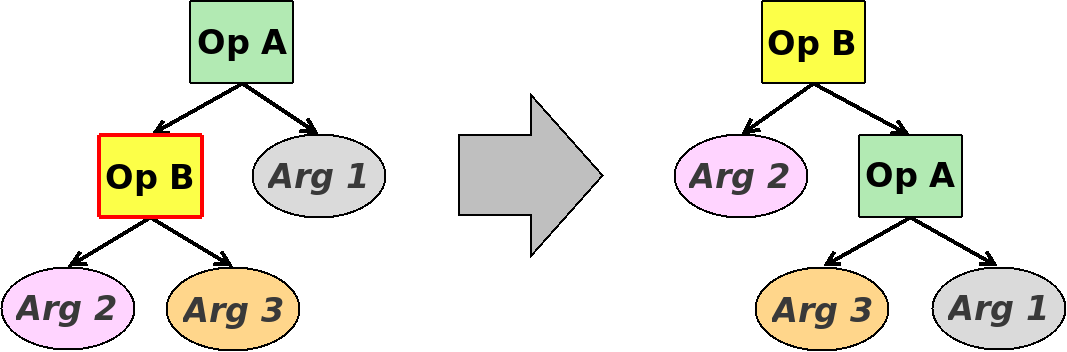
\includegraphics[width=250pt, height=82pt]{./rotacion1.png}
\caption{\label{rotacion1} Caso de rotación cuando la operación de la izquierda tiene menor precedencia.}
\end{figure}

\begin{figure}[!ht]\centering
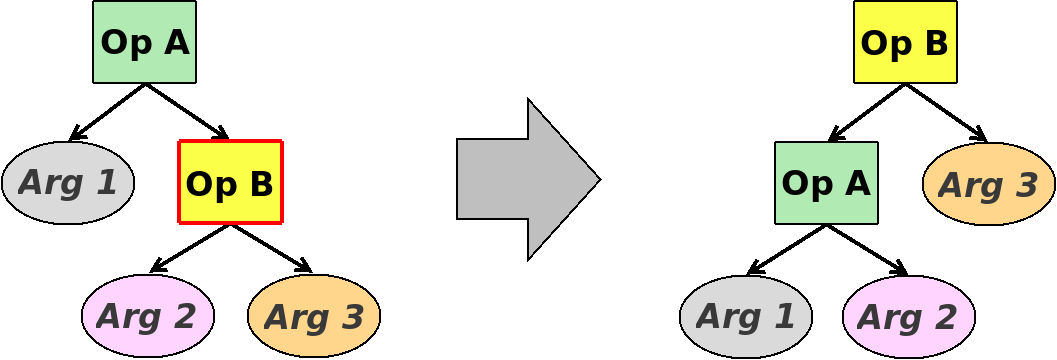
\includegraphics[width=250pt, height=85pt]{./rotacion2.png}
\caption{\label{rotacion2} Caso de rotación cuando la operación de la derecha tiene menor precedencia.}
\end{figure}

\item En cambio, cuando se inserta cualquier operación como hija de una operación prefija (raíz) y la insertada tiene mejor precedencia que la raíz, no se resuelve instantáneamente el error, dado que se alteraría el orden sintáctico de la expresión. Para ello se prende una bandera, a la cual se le asigna el valor de precedencia que tiene la operación recién insertada. Entonces cuando en el siguiente paso se agregue una nueva raíz, si tiene mayor precedencia que su ``nieto'' en el árbol, se realiza la siguiente rotación mostrada en el diagrama \ref{rotacion3}.

\begin{figure}[!ht]\centering
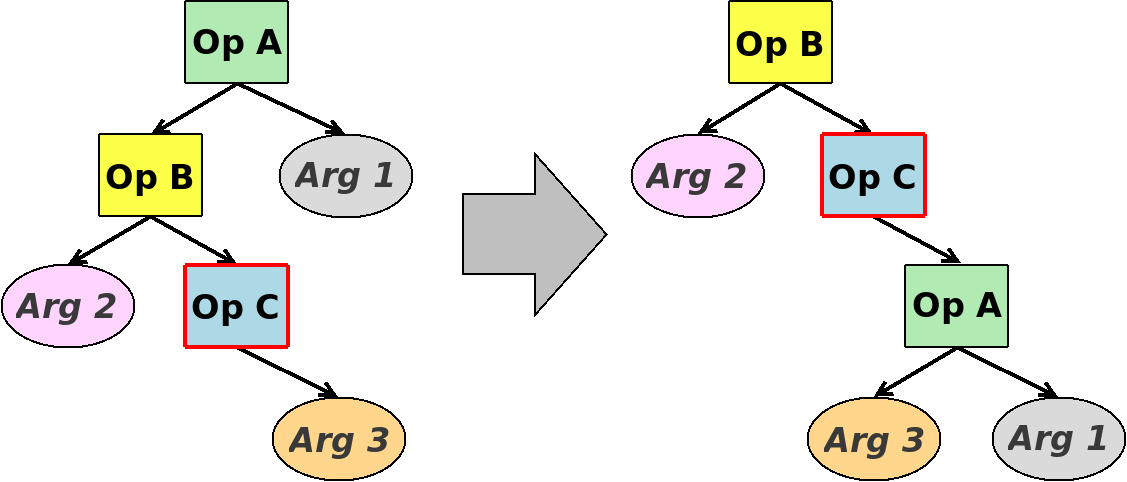
\includegraphics[width=250pt, height=107pt]{./rotacion3.png}
\caption{\label{rotacion3} Caso de rotación cuando se detectó un conflicto sin resolver.}
\end{figure}
\end{itemize}

\subsection{Asociatividad de operadores dentro de expresiones}

El chequeo de la asociatividad y las eventuales modificaciones en el árbol de expresión, a diferencia del tratamiento que se le da a los problemas de precedencia, no se realiza a medida que se obtiene el árbol, sino que se lo aplica solamente una vez, cuando ya se terminó de parsear la expresión.

Esto se implementó así, ya que en ese punto, todos los elementos del árbol se encuentran posicionados respetando todas las precedencias, quedando potencialmente inconsistente la asociación de dos o más operadores infijos iguales, dentro del mismo nivel sintáctico, y con asociatividad a \textbf{derecha}, ya que por defecto todos los operadores son asociados a izquierda, debido al parser descendente recursivo que aplica \spirit.

Además, cuando se detectan dos operadores no asociativos se genera un error por mal uso de ese operador dentro de la expresión. Tal como se analizó en la sección \ref{subsubsec:operconsi}.

\subsection{Alcanzabilidad de símbolos y reglas}

En la especificación pueden existir símbolos y reglas declaradas que no pueden ser alcanzados desde el símbolo inicial de la gramática. Los mismos no son útiles en la gramática ya que nunca producirán cadenas del lenguaje. Los mismos no son considerados errores pero son informados mediante alertas (\textbtt{warnings}).

Este chequeo se implementó con una versión del algoritmo de Warshall\footnote{En honor a Stephen Warshall (1935-2006)}, que calcula la ``\textit{Clausura Transitiva}'' de un grafo.

Para aplicarlo, primero se construye una matriz de valores lógicos reflejando todas las reglas declaradas. Luego de computar la clausura, se recorre la fila del símbolo inicial, que pertenece a la \textbf{única} regla inicial de la gramática por ser \textbf{extendida}. Todo símbolo que se encuentra con valor falso es inalcanzable.

\subsection{Consistencia de bloque de atributos y bloque de reglas}

Este chequeo consiste en verificar que no existan símbolos declarados en el bloque de atributos, que no hallan sido involucrados en ninguna regla. Esto puede suceder cuando se crearon los símbolos de la expresión de conjuntos que define la pertenencia de un atributo.

La heurística utilizada, consiste en recorrer el \textbtt{map} de símbolos no terminales y verificar que existe al menos una regla que lo tenga como parte izquierda.

\subsection{Gramática bien definida}

Este control es uno de los más importantes, ya que si la gramática por más que haya sido parseada correctamente, si no cumple con las condiciones de una MAG, la herramienta la descarta y no le generará su correspondiente evaluador.

Como ya se mencionó en la sección \ref{subsec:check}, varias son las condiciones que se deben chequear.

La heurística aplicada fue recorrer el \textbtt{map} de reglas, donde para cada una se verificaba que estuviesen definidas dentro de su \textbtt{map} de ecuaciones, una para cada uno de sus atributos sintetizados. Y a su vez, una ecuación para cada atributo heredado de sus símbolos de la parte derecha.

Además, también se controlara que no existieran ecuaciones incorrectas, es decir:
\begin{itemize}
\item Ecuaciones para atributos heredados del símbolo de la izquierda.
\item Ecuaciones para atributos sintetizados de símbolos de la parte derecha.
\end{itemize}

Cada vez que se detectaba un error, se lo informa mediante alguno de los siguientes mensajes según corresponda.
\footnotesize{\textbtt{\begin{items}
\item ERROR: ``E[1].syn1'' type synthetized, haven't an equation that defines it.
\item ERROR: ``S[0].inh1'' type inherited, is defined outside his scope.
\item ERROR: ``E[1].inh2'' type inherited, haven't an equation that defines it.
\item ERROR: ``S[0].syn2'' type synthetized, is defined outside his scope.
\end{items}}}

\section{Obtención de planes de evaluación}
\label{sec:obtplaneval}

El propósito final de \maggen\ es obtener todos los planes posibles de la gramática de entrada. En la sección \ref{subsec:conts-plan-dise}, se analizaron algunas consideraciones a tener en cuenta, en esta sección las se retoman desde el punto de vista de la implementación. 

Teóricamente un plan es una secuencia de instancias, que indica un orden de evaluación total y consistentes de las mismas. Dentro de \maggen, se optó para su representación una secuencia de identificadores de ecuaciones. Ya que cada ecuación tiene solamente \textbf{un} \textbtt{l\_value}, que es precisamente una instancia. Se utiliza la clase \textbtt{vector} de la STL, para su almacenamiento y están enumeradas de forma tal que pueden ser identificadas de manera univoca.

Como en general, se iban a generar en muchos casos los mismos planes, se decidió mantener un \textbtt{vector} con todos los planes diferentes, así solo se generarían la \textbf{mínima cantidad de planes}, es decir, únicos necesarios.

Como en el algoritmo que se presenta en el artículo de Wuu Yang (\cite{wuu-yang1}), a cada plan se lo asocia con un \textbtt{key}, primero se implementó esa clave como una estructura con los siguientes datos:
\begin{itemize}
\item La regla a la cual pertenece el plan
\item Una secuencia para computar sus atributos
\end{itemize}

Esa secuencia se representó de igual manera que un plan, ya que computar un atributo es equivalente a saber el identificador de la ecuación que lo tiene como \textbtt{l\_value}.

El conjunto de estas secuencias, son los planes proyectados, es decir, las exigencias que se le imponen a una regla desde un contexto superior que la invoca a que se compute. Para el símbolo inicial, esta secuencia es obtenida como el orden topológico de su grafo DCG, ya que este contiene todas las dependencias entre los atributos de la regla, el cual si o si, será un orden de computación consistente para sus ecuaciones.

Al igual que con los planes de evaluación, los planes proyectados también sufrían de muchas repeticiones, por lo cual se usaron índices indirectos a un repositorio de los mismos almacenados en un \textbtt{vector}.

Cada plan proyectado estaba bajo una clave particular, la cual según el algoritmo debía contener:
\begin{itemize}
\item La regla a la cual pertenece el plan proyectado
\item Una secuencia para computar sus atributos
\item El símbolo con el cual se proyectó el plan de evaluación
\end{itemize}

Los dos primeros valores, corresponden a un \textbtt{key} de un plan de evaluación, así que se usó directamente esa estructura.

\subsection{Construcción de grafos}
\label{subsec:const-graf}
Para la representación de los grafos se utilizó la \boost\ \textit{\textbf{Graph Library}} (\textbf{BGL}). Ya que la misma presentaba muchas funcionalidades y ya se encontraba como una dependencia externa de la herramienta (debido a que \spirit\ forma parte de \boost, como ya se mencionó al principio del capítulo).

Como en la mayoría de los componentes de esta biblioteca, los mismos eran plantillas que necesitaban ser instanciados.

Las dependencias dentro de las reglas se dan entre las instancias de atributos de las ecuaciones y además los literales.

En la \textbf{BGL} los valores que se quieren asociar a los nodos, se vinculan mediante \textit{propiedades} inherentes a cada uno.

\begin{lstlisting}[columns=fullflexible, basicstyle=\scriptsize, linewidth=13.5cm]
struct vertex_data_t
{
  typedef vertex_property_tag kind;
};
typedef property <vertex_data_t, const genevalmag::Expr_leaf*> property_vertex_dp;
typedef adjacency_list <hash_setS, vecS, directedS, property_vertex_dp> Graph;
typedef Graph::vertex_descriptor Vertex;
\end{lstlisting}

Se mantienen dentro de la herramienta un \textbtt{map} para cada uno de los tipos de grafos necesarios y además para los subgrafos ADP cíclicos que eventualmente se detecten y para optimizar la construcción de los otros, los grafos que contienen todas las instancias de cada regla sin aristas entre si.

\begin{lstlisting}[basicstyle=\scriptsize, linewidth=10.7cm]
map <string, Graph>                 attr_vertex_graphs;
map <unsigned short, Graph>         p_Dp_graphs;
map <string, Graph>                 p_Down_graphs;
map <unsigned short, Graph>         p_Dcg_graphs;
map <vector<unsigned short>, Graph> p_Adp_graphs;
map <vector<unsigned short>, Graph> p_Adp_subgraphs_cyclics;
\end{lstlisting}

\subsection{Ciclicidad}

El chequeo de ciclicidad sobre los grafos ADP, se implementó utilizando el algoritmo de búsqueda en profundidad (Depth-first search) de \boost\ combinado con la creación de un ``visitador'' especializado. El cual a medida que recorre el grafo, va guardado los nodos y aristas visitadas mientras no se halla detectado un ciclo. Ese subgrafo es mostrado al usuario en caso de error, sino es descartado.

La detección de ciclos, se ejectua cuando el algoritmo de visite, invoca a la función \textbtt{back\_edge}, en el cual es activada la bandera que indice este suceso.

Tanto el grafo como la variable lógica, usada como bandera, son pasadas en el constructor y utilizadas internamente mediante referencias.

\begin{lstlisting}[columns=fullflexible, linewidth=9.2cm]
struct cycle_detector: public dfs_visitor<>
{
  public:
    cycle_detector(bool& has_cycle, Graph &graph):
      _has_cycle(has_cycle), 
      _graph_cycle(graph)
    {}

    template <class Edge, class G>
    void examine_edge(Edge u, const G &g)
    {
      if(!_has_cycle)
      {
         ...
      }
    }

    template <class Edge, class G>
    void back_edge(Edge u, const G& g)
    {
      _has_cycle = true;
    }

  protected:
    bool   &_has_cycle;
    Graph  &_graph_cycle;
};
\end{lstlisting}

\subsection{Contextos}

Para cada regla, se tienen que considerar todos los posibles contextos inferiores de acuerdo a las reglas que tengan los símbolos no terminales de su parte derecha. Se implementó un método que recursivamente genera un contexto diferente y guarda la regla cuando ya no quedan más variantes.

\subsubsection{Unicidad de contextos, planes y planes proyectados}

Al igual que con los planes, los contextos de las reglas se repiten mucho, así que se utilizaron índices indirectos sobre un \textbtt{vector} que almacena únicamente los contextos diferentes.

\begin{lstlisting}[numbers=left, linewidth=9cm]
vector <Order_rule>    contexts_uniques;
vector <Order_eval_eq> plans_uniques;
vector <Order_eval_eq> plans_project_uniques;
\end{lstlisting}

Antes de insertar un elemento en cualquiera de estos repositorios se verifica que no exista. En caso de que ya se encuentre, se devuelve el índice correspondiente dentro del vector, sino se insertará al final y se devolverá el índice del último elemento.

\subsection{Representación en Dot}

Una vez que se generaron todos los tipos de grafos, los mismos son guardados en distintos directorios en formato \textbf{DOT}\cite{dot} (detalles sobre las salidas de \maggen pueden analizarse en el capítulo \ref{chap:usos}). Para generar las especificaciones en el lenguaje DOT se utilizó la función \textbtt{write\_graphviz} perteneciente al módulo Graphviz de \boost.

\subsection{Generación de grafos}

La generación de grafos es incremental, partiendo de la computación de los grafos DP, siguiendo los Down, DCG y por último los grafos ADP. Ante cualquier fallo, la generación se considerará incompleta.

\begin{lstlisting}[numbers=left, columns=fullflexible, linewidth=11.3cm]
bool generate_graphs()
{
  if(build_graphs.compute_dependency_graphs())
  {
    if(build_graphs.compute_down_graph())
    {
      if(build_graphs.compute_dcg())
      {
        if(build_graphs.compute_adp_graph())
        {
          cout << "* Generate graphs ---------- [  OK  ]" << endl;
          return true;
        }
      }
    }
  }
  cout << "* Generate graphs ---------- [ FAIL ]\n" << endl;
  return false;
}
\end{lstlisting}

\subsection{Generación de planes}
\label{sec:genplanes}

Una vez que se concluyó la generación de grafos, se prosigue con el chequeo de ciclicidad de los grafos ADP. Si se supera con éxito, se generarán los planes, sino se abortará el proceso.

\begin{lstlisting}[numbers=left, columns=fullflexible, linewidth=11.7cm]
unsigned short build_plans()
{
  if(generate_graphs())
  {
    if (build_graphs.check_cyclic_adp_dependencies())
    {
      cout << "* Build plans -------------- [ ABORT ]\n" << endl;
      return 1;
    }
    else if(generate_plans())
    {
      cout << "* Build plans -------------- [  OK  ]" << endl;
      return 0;
    }
    cout << "* Build plans -------------- [ FAIL ]\n" << endl;
  }
  return 2;
}
\end{lstlisting}

El proceso de construir un plan es complejo, la heurística seguida respeta el algoritmo para computar planes presentado por Wuu Yang (\cite{wuu-yang1}).

Por lo que se implementaron las funciones y elementos involucrados que se pueden analizar en la tabla \ref{table:map-comp-plan}.
\begin{table}[!ht]
\begin{tabular}{| p{4.5cm} | p{9.5cm} |}
\hline
Lista de trabajos \textbf{WL} & \textbtt{vector <Item\_work>\ work\_list} \\ \hline

Trabajos realizados {\LARGE\textbf{$\Delta$}} & \textbtt{vector <Item\_work>\ defined\_item\_work} \\ \hline

Función \textbf{ComputeOrder} de ecuaciones & \textbtt{compute\_order (const Graph \&graph\_adp, unsigned short index\_order, const Context\_rule \&context\_rule)} \\ \hline

Función \textbf{Project} orden de ecuaciones para un símbolo & \textbtt{purge\_plan\_with (const Rule \&rule, const Order\_eval\_eq \&order\_eq, Order\_eval\_eq \&purged\_order)} \\ \hline

Planes de evaluación {\LARGE\textbf{$\Theta$}} & \textbtt{map <Key\_plan, unsigned short>\ eval\_plans} \\ \hline

Planes de evaluación \hspace{1cm}proyectados {\LARGE\textbf{$\gamma$}} & \textbtt{map <Key\_plan\_project, unsigned short>\ plans\_project} \\
\hline
\end{tabular}
\caption{\label{table:map-comp-plan} Implementación de funciones en Compute Plan}
\end{table}

Para la función \textbtt{compute\_order} se debe considerar el orden de evaluación de los atributos establecido por el \textbtt{index\_order}, el cual es el índice de un plan proyectado. Por lo que, primero se crea un grafo ADP copiando el grafo referenciado por \textbtt{graph\_adp}, luego se le insertan los vértices necesarios, utilizando la función \textbtt{return\_vertex}\footnote{Función que dado un atributo retorna un \textbtt{vertex\_descriptor} de un vértice existente dentro del grafo o sino lo inserta y retorna un nuevo descriptor.} y se insertan las aristas entre los atributos consecutivos.

Por ejemplo para este orden de atributos:
\vspace{0.1cm}
\begin{center}
\Large\textbf{$a_{4}, a_{2}, a_{0}, a_{1}, a_{5}, a_{6}, a_{3}$}
\end{center}
\vspace{0.2cm}
Se insertarán las siguientes 6 aristas, que podían ya existir dentro del grafo:
\vspace{0.1cm}
\begin{center}
\Large\textbf{$a_{4} \rightarrow a_{2}, a_{2} \rightarrow a_{0}, a_{0} \rightarrow a_{1}, a_{1} \rightarrow a_{5}, a_{5} \rightarrow a_{6}, a_{6} \rightarrow a_{3}$}
\end{center}
\vspace{0.2cm}

Luego se le aplica la función \textbtt{warshall\_transitive\_closure}, que computa la clausura transitiva del grafo, perteneciente a la \textbf{BGL} de \boost. Esto causa que ese orden inducido por los atributos repercuta en todos los componentes del grafo.

Por último, mediante la función \textbtt{generates\_topological\_order}, que como su nombre lo indica calcula el orden topológico del grafo, se obtiene el orden de evaluación consistente de las ecuaciones de la regla actual.

La función \textbtt{purge\_plan\_with}, dado un plan de evaluación de ecuaciones, para una cierta regla, y otra regla, devuelve un nuevo plan, conteniendo las ecuaciones de ese plan que pertenecen a la otra regla pasada como parámetro.

\section{Construcción de Secuencias de Visita}

Este proceso como se explicó en la sección \ref{sec:constseqvisit}, consiste en lograr a partir de cada plan de evaluación, su correspondiente traducción a una secuencia de visita consistente, que permita navegar el árbol al momento de la evaluación. La misma esta compuesta, básicamente, por tres valores:

\begin{itemize}
\item \textbtt{Visit}: visitar a un nodo hijo debido a que necesita que le compute algún atributo sintetizado.
\item \textbtt{Leave}: vuelve a su ancestro (padre), debido a que necesita que le calculen algún atributo heredado.
\item \textbtt{Compute}: se encuentra en condiciones de computar uno de sus atributos sintetizados o heredado de sus hijos.
\end{itemize}

Por la forma de los mismos, se decidió como forma de representación un arreglo de enteros, con el siguiente criterio:

\begin{itemize}
\item $\textbtt{Visit}\ \ \ \  \Rightarrow \ \ \textbf{>0}$: Números positivos indican que nodo hijo se debe visitar, arrancando en 1 para el primero.
\item $\textbtt{Leave}\ \ \ \  \Rightarrow \ \ \textbf{=0}$: El cero indica que se tiene que volver al padre del nodo.
\item $\textbtt{Compute} \Rightarrow \ \textbf{<0}$: Números negativos indican que ecuación debe computarse, tomando obviamente el valor absoluto y respetando la numeración global de las mismas.
\end{itemize}

La cantidad de secuencias de visitas es la misma que la de los planes de evaluación generados, y como este proceso se apoya en una ``\textbf{simulación}'', la construcción de las secuencias se da en forma incremental. Por eso se inicializan todas las estructuras de almacenamiento con secuencias de visitas vacías, que luego serán modificadas mediante indexación sobre el repositorio.

Aquí queda claro la optimización realizada mediante la creación de planes únicos, es decir, no existen dentro de \maggen\ planes repetidos. Por lo tanto, sólo se crearán una cantidad mínima de secuencias de visita también. 

% Para ver cifras de la optimización, dirigirse al capítulo \ref{XXX}.

La implementación fue la siguiente:

\begin{lstlisting}[columns=fullflexible, linewidth=7cm]
typedef vector < int > Visit_seq;

vector < Visit_seq > all_visit_seqs;
\end{lstlisting}

\subsection{Heurística de la simulación: Detalles de implementación}

Como ya se analizó en la sección \ref{subsec:heuris-simul}, con la heuristica utilizada,  basta con lanzar el proceso de simulación sobre él o los planes asociados a la regla inicial. Además es correcto, porque toda evaluación comenzará desde ese punto.

El algoritmo que se diseñó es recursivo y se apoya en ciertas listas que llevan información de contextos anteriores que son utilizados para realizar podas\footnote{Heurística que permite descartar ramas completas en problemas sobre decisión en árboles y grafos análogamente. \urllink{http://en.wikipedia.org/wiki/Branch\_and\_cut}} y cálculos innecesarios. Estos son:

\begin{description}
\item [Instancias Computadas:] referencia a las instancias de atributos que ya se calcularon en algún contexto.
\begin{lstlisting}
vector<Expr_instance> &ins_computed
\end{lstlisting}

\item [Planes Computados:] referencia a los planes de evaluación ya traducidos por completo.
\begin{lstlisting}
vector< map<Key_plan, unsigned short>::const_iterator > &plans_computed
\end{lstlisting}

\item [Secuencias de Visita Computadas:] referencia a las secuencias de visita que ya fueron calculadas completamente.
\begin{lstlisting}
vector<unsigned short> &v_seq_computed
\end{lstlisting}
\end{description}

El algoritmo principal, \textbtt{generate\_visit\_sequences}, es más bien un invocador de la función \textbtt{gen\_visit\_seq}, que es la que realmente lleva a cabo las llamadas que simulan la evaluación.

\begin{lstlisting}[numbers=left, columns=fullflexible]
bool generate_visit_sequences()
{
  for(size_t i(0); i < b_plans.get_plans_uniques().size(); i++)
  {
    Visit_seq v_s;
    all_visit_seqs.push_back(v_s);
  }

  vector <unsigned short> visit_seq_computed;
  vector <map <Key_plan, unsigned short>::const_iterator> plans_computed_all;
  /* For all plans */
  for(map <Key_plan, unsigned short>::const_iterator it(b_plans.get_plans().begin()); it != b_plans.get_plans().end(); it++)
  {
    const Rule &rule(attr_grammar.get_rule(b_plans.get_context_unique(it->first.id_plan)[0]));
    if (rule.get_left_symbol()->equals(*attr_grammar.get_initial_symb()))
    {
      /* This plan is belong a initial symbol (initial rule). */
      if(!belong_index(it->second, visit_seq_computed))
      {
        vector <Expr_instance> ins_computed;
        vector <map <Key_plan, unsigned short>::const_iterator> plans_computed;
        merge_vec(plans_computed_all, plans_computed);
        gen_visit_seq(it, ins_computed, plans_computed, visit_seq_computed);
        merge_vec(plans_computed, plans_computed_all);
        plan_family_computed(plans_computed, visit_seq_computed);
      }
    }
  }
  cout << "* Build visit sequence ----- [  OK  ]" << endl;
  return true;
}
\end{lstlisting}

Dentro de \textbtt{gen\_visit\_seq}, se recorre el plan de evaluación respetando los criterios explicados en \ref{sec:constseqvisit}. Además se debe asegurar que sólo se actualice la secuencia de visita correspondiente al plan actual,si no se produjo ningún \textbtt{leave}. Para ello se lleva una variable lógica (flag) que indica la ausencia de \textbtt{leaves}, además una secuencia de visita y un listado de instancias de atributos computados a nivel local.

Durante su funcionamiento se cumplen las siguientes condiciones:
\begin{itemize}
\item Los atributos sintetizados del símbolo de la izquierda de la regla, son informados a nodo padre, mediante su inserción en \textbtt{ins\_computed} pasado como referencia.

\item Los atributos ya sean sintetizados del símbolo de la izquierda o heredados de algún símbolo de la derecha, son insertados en \textbtt{ins\_computed\_own}.

\item Siempre que se termina de recorrer un plan, se actualiza la secuencia de visita del plan actual siempre y cuando no pertenezca a \textbtt{v\_seq\_computed}.

La actualización se lleva a cabo mediante la función \textbtt{update\_visit\_sequence}, la cual:
\begin{items}
\item Recibe un índice que representa tanto a un plan como a su secuencia de visita y una secuencia de visita ``nueva''.

\item Empareja la vieja secuencia, verificando posición a posición que sean iguales, pero si en la secuencia ya guardada existe un \textbtt{leave}, es decir, un cero, vuelve a avanzar.

\item Termina cuando encuentra diferencias o cuando llega al final de alguna de las dos secuencias.

\item Por último, actualiza la secuencia guardada insertando los valores restantes que hayan quedado de la nueva secuencia.
\end{items}

\underline{Por ejemplo:}\hspace*{1cm} \textbf{[-7, 0]} update con \textbf{[-7, -8]}\\
\hspace*{2.8cm} da como resultado: \textbf{[-7, 0, -8]}\footnote{Secuencia de visita del ejemplo del apéndice \ref{append:agwuuyang}}.

\item Si un plan se recorrió en su totalidad, se inserta en \textbtt{plans\_computed}.

\item La instancia que se encuentra en el \textbtt{l\_value} de la ecuación, será marcada con un \textbtt{compute} solamente cuando se haya podido consumir el \textbtt{r\_value} de la ecuación y no se haya dado un \textbtt{leave}.

\item Cuando se debe realizar un \textbtt{visit}

\begin{items}
\item Se obtiene de la instancia de atributo, es número de ocurrencia, que sirve para identificar al nodo hijo a visitar.

\item Una vez localizado, se busca el plan proyectado para ese símbolo bajo el contexto actual.

\item Luego se inserta en la secuencia de visita local el \textbtt{visit}.

\item Se invoca recursivamente a \textbtt{gen\_visit\_seq} con:

\begin{items}
\item \textbtt{ins\_computed\_child}: inicializado con todos los atributos heredados del símbolo a recursar, calculados hasta el momento.

\item \textbtt{p\_computed\_child}: inicializado con todos los planes computados hasta el momento, más el índice del plan actual ``virtualmente'' ya computado para evitar ciclos de llamadas recursivas.

\item \textbtt{v\_seq\_child}: inicialmente está vacío para la recursión del primer plan seleccionado, pero es acumulativo para las demás llamadas. Indica las secuencias de visita ya calculadas.
\end{items}

\item Al terminar la recursión, la \textbtt{gen\_visit\_seq} (invocación), se extraen los resultados útiles para este contexto.

\begin{items}
\item Nuevos planes computados a partir de la llamada sobre el nodo hijo, exceptuando la ``computada virtual'' del plan actual. Insertados en \textbtt{plans\_computed}.

\item Nuevos atributos sintetizados calculados del nodo hijo. Insertados en \textbtt{ins\_computed\_own}.

\item Nuevas secuencias de visitas obtenidas completamente. Insertados en \textbtt{v\_seq\_child}.
\end{items}
\end{items}

\end{itemize}


\section{Generación de código}

Esta es la última etapa de \maggen\ y la que produce el resultado esperado por el usuario: el código fuente en C++ de un Evaluador para la gramática que especificó en el archivo de entrada.

Es un proceso que debe dejar plasmado en código estático todos los resultados obtenidos durante las anteriores etapas.

Para obtener un diseño dentro de los estándares de C++, se crean dos archivos: una cabecera \textbtt{.hpp} y un fuente \textbtt{.cpp}. Ambos archivos son creados con el nombre proporcionado por el usuario mediante la opción \textbtt{maggen -o name} o sino con el nombre por defecto: \textbtt{mag\_eval}\footnote{Para más detalles sobre usos, ver capítulo \ref{chap:usos}.}.

También se copian al directorio de salida de \maggen, dos archivos utilizados por el evaluador:
\begin{items}
\item \textbtt{Node.hpp:} ver código fuente en apéndice \ref{append:nodehpp}
\item \textbtt{Plan.hpp:} ver código fuente en apéndice \ref{append:planhpp}
\end{items}

\vspace*{0.2cm}

La generación de código es un proceso reiterativo sobre cada elemento almacenado en los repositorios de la herramienta. Por ejemplo, la función que produce el código que representa a un símbolo, se aplicará sobre cada uno de ellos.

La función principal es \textbtt{generate\_code}, en donde se invocan a las demás funciones para generar los fuentes del evaluador.

\begin{lstlisting}[numbers=left, columns=fullflexible, linewidth=11.5cm]
bool generate_code(const vector<string> &headers_file) const
{
  generate_header_file();
  generate_code_file(headers_file);

  generate_structs();
  generate_constructor();
  generate_methods();

  generate_footer_header();
  generate_footer_code();

  if (!copy_static_code(path_output))
  {
    cout << "* Generation code ---------- [ FAIL ]" << endl;
    return false;
  }

  cout << "* Generation code ---------- [  OK  ]" << endl;
  return true;
}
\end{lstlisting}

Notar que recibe como parámetro una referencia a los ``\textbtt{headers}'' que el usuario proporcionó en el momento de la invocación de \maggen \footnote{Ver sección \ref{sec:uso-maggen} para obtener detalles sobre parametros de invocación.}. Los mismos serán incluidos en el archivo \textbtt{.cpp}.

\subsection{Cabecera del evaluador}

Dentro de este archivo, se definen para cada \textbf{símbolo no terminal} una tipo en base a una estructura que incluye a sus atributos, un constructor y un método \textbtt{to\_string()} que genera una cadena con su estado actual.

\underline{Por ejemplo:} símbolo Y, del ejemplo de Wuu Yang en el apéndice \ref{append:agwuuyang}.
\begin{center}\textbtt{symbol Y  NonTerminal Attributes: i2, i3, s2, s3;}\end{center}
se define lo siguiente:
\begin{lstlisting}[columns=fullflexible, linewidth=7.3cm]
typedef struct Symbol_Y: Node
{
    int i2;
    int i3;
    int s2;
    int s3;

    Symbol_Y(const unsigned short &r_id);

    string to_string() const;
} Y ;
\end{lstlisting}

Luego de realizar ciertos análisis, se determinó que realmente varias estructuras que eran vitales en fases anteriores, ahora en el contexto y funcionamiento del evaluador eran innecesarias. Por ejemplo, de los planes de evaluación y planes proyectados, únicamente se utilizan los índices de los mismos. Esto sucede ya que debido a la optimización de generar sólo planes diferentes e indexarlos, no existe necesidad de tener en forma estática la definición de cada uno de ellos.

En cambio, las secuencias de visitas son imprescindibles para la evaluación, como así también una versión reducida de las definiciones de las reglas, incluyendo solamente un arreglo con los nombres de cada símbolo no terminal que participa en la misma, en donde la posición cero corresponde al símbolo \textbtt{head} y las demas posiciones al \textit{body}\footnote{Ver \ref{sec:def-CFG}}.

Aquí se incluyen los perfiles de los métodos públicos y privados mencionados en \ref{sec:gencodigo}.

\subsection{Fuente del evaluador}

Lo primero que el ``desarrollador\footnote{Un usuario que se interesa en indagar el código del evaluador.}'' se encuentra al abrir este archivo, es la implementación del constructor y del método \textbtt{to\_string()} de cada uno de los símbolos no terminales. Por cuestiones del diseño realizado, cada nodo del AST tiene un identificador de regla, que debe ser un \textbf{número positivo mayor que cero}.

A modo de ejemplo, se muestra el código C++ generado para el símbolo Y, del ejemplo de Wuu Yang en el apéndice \ref{append:agwuuyang}.

\begin{lstlisting}[columns=fullflexible, linewidth=9.3cm]
Y::Symbol_Y(const unsigned short &r_id): Node(r_id){}

string Y::to_string() const
{
  string text("-- Values of symbol Y:\n");
  text.append("     - Attribute inherited i2 = ");
  stringstream str_i2;
  str_i2 << i2;
  text.append(str_i2.str());
  text.append("\n");
  text.append("     - Attribute inherited i3 = ");
  stringstream str_i3;
  str_i3 << i3;
  text.append(str_i3.str());
  text.append("\n");
  text.append("     - Attribute synthesized s2 = ");
  stringstream str_s2;
  str_s2 << s2;
  text.append(str_s2.str());
  text.append("\n");
  text.append("     - Attribute synthesized s3 = ");
  stringstream str_s3;
  str_s3 << s3;
  text.append(str_s3.str());
  text.append("\n");
  for(size_t i(0); i < childs.size(); i++)
  {
    text.append(childs[i]->to_string());
  }
  return text;
}
\end{lstlisting}

Toda las estructuras son inicializadas en el constructor del evaluador, las mismas son:

\begin{itemize}
\item Contextos:
\begin{lstlisting}[columns=fullflexible]
unsigned short __context_0[] = {1, 4, 2, 5};
Order_rule context_0(__context_0, __context_0 + sizeof(__context_0) / sizeof(unsigned short));
contexts_rule.push_back(context_0);
\end{lstlisting}

\item Planes de evaluación:
\begin{lstlisting}[columns=fullflexible, linewidth=4.5cm]
Key_plan key_0(0, 0);
add_plan(key_0 , 0);
\end{lstlisting}

\item Planes de evaluación proyectados:
\begin{lstlisting}[columns=fullflexible, linewidth=9.5cm]
Key_plan key_plan_proj_0(0, 0);
Key_plan_project key_proj_0(key_plan_proj_0, 2, 0);
add_plan_project(key_proj_0 , 1);
\end{lstlisting}

\item Secuencias de visita:
\begin{lstlisting}[columns=fullflexible]
int __order_0[] = {2, -2, 1, -3, 2, -4, 3, -1};
Visit_sequence order_0(__order_0, __order_0 + sizeof(__order_0) / sizeof(int));
v_seq.push_back(order_0);
\end{lstlisting}

\item Reglas:
\begin{lstlisting}[columns=fullflexible]
unsigned short __rule_non_terminal_0[] = {1, 2, 3, 4};
Rule rule_non_terminal_0(__rule_non_terminal_0, __rule_non_terminal_0 + sizeof(__rule_non_terminal_0) / sizeof(unsigned short));
rules.push_back(rule_non_terminal_0);
\end{lstlisting}
\end{itemize}

La mayor parte de los algoritmos utilizados dentro del evaluador generado, se encuentran escritos dentro de la herramienta y son transcritos al archivos fuente directamente.

\subsection{Algoritmo de evaluación}
\label{sec:codcppalgeval}

El algoritmo que se implementó para poder evaluar un AST, es el propuesto por Wuu Yang en \ref{sec:algevalattr}. El cual realiza dos etapas bien definidas:

\begin{description}
\item [Primera recorrida del AST] se invoca a la función
\begin{items}
\item \textbtt{traverse}: responsable de seleccionar el plan de evaluación para cada nodo no terminal.
\end{items}

\item [Segunda recorrida del AST] se invoca a la función
\begin{items}
\item \textbtt{eval\_visiter}: es un evaluador orientado a visitas, que debe computar los valores de los atributos de los nodos.
\end{items}
\end{description}

El código del evaluador es reducido por su gran nivel de modularización. Recibe como parámetro la raíz del AST a evaluar. El orden inicial de evaluación para los atributos del símbolo inicial y, que por ser una gramática extendida no ocurre en ningún otro lado de la misma, siempre se encuentra en la posición cero del arreglo de planes de evaluación únicos.

\begin{lstlisting}[numbers=left, columns=fullflexible, linewidth=6.8cm]
void evaluator_mag(struct Node *root)
{
    unsigned short order_init(0);
    traverse(root, order_init);
    eval_visiter(root);
}
\end{lstlisting}

\subsubsection{Función Traverse}
\fbox{\textbtt{\textbf{void traverse (struct Node *node, unsigned short order)}}}\\

Esta función a partir del identificador de regla que posee cada nodo AST, construye un \textbtt{Order\_rule}, es decir, su contexto de invocación. Luego, mediante la función \textbtt{return\_index\_context} se obtiene su índice relativo dentro del arreglo que contiene a todos los contextos únicos computados por \maggen. Si no lo encuentra, produce un error ya que el AST de entrada posee un contexto incorrecto para la gramática para la cual se generó el evaluador.

Después se arma un \textbtt{Key\_plan} con dicho índice y el parámetro \textbtt{order}, que es el índice del plan proyectado que se corresponde con el orden de evaluación de sus ecuaciones, impuesto por su contexto superior.

Por último se busca el plan de evaluación correspondiente al nodo visitado y se lo guarda en la estructura del nodo en el campo \textbtt{visit\_seq\_index}.

Ahora se debe visitar a cada uno de los hijos, imponiéndole a los mismos un orden específico para que evalúen sus atributos según dependencias que inducen dicho orden.

Para lo cual se tiene que elegir el plan proyectado utilizando el plan seleccionado del nodo actual, el identificador de regla del hijo a visitar y el símbolo no terminal que representa en el \textbf{body}\footnote{Ver \ref{sec:def-CFG} definición de \textbf{CFG}.} de la ecuación.

Por lo cual se construye lo siguiente para buscarlo dentro del vector de planes proyectados únicos:

\begin{center}\textbtt{Key\_plan\_project k\_plan\_proj(k\_plan, rule[i+1], i)}\end{center}

donde la variable ``\textbtt{i}'' se desplazará desde 1 a la cantidad de hijos\footnote{La cantidad de hijos es idéntica a la longitud de la regla que representa al nodo.}.\\

Con lo cual se realiza la llamada recursiva de la función:

\begin{center}\textbtt{traverse(node->childs[i], eval\_plans\_project[j].second);}\end{center}

donde ``\textbtt{j}'' corresponde al índice del plan proyectado del hijo a visitar.
\subsubsection{Función Eval}
\fbox{\textbtt{\textbf{void eval\_visiter(struct Node *root)}}}\\

Esta función sigue los lineamientos de la secuencia de visita referenciada por cada nodo. Arrancando desde la raíz, el algoritmo dirige la evaluación del AST para lograr el AST decorado.

\begin{lstlisting}[numbers=left, columns=fullflexible]
void eval_visiter(struct Node *root)
{
  for(size_t i(root->pos_visit_seq); i < v_seq[root->visit_seq_index].size(); i++)
  {
    int item_visit(v_seq[root->visit_seq_index][i]);
    if (item_visit > 0)
    {
      eval_visiter(root->childs[item_visit - 1]);
    }
    else if (item_visit < 0)
    {
      compute_eq((item_visit * (-1)), root);
    }
    else
    {
      /* Saves the index of the current v_seq item. */
      root->pos_visit_seq = i+1;
      return;
    }
  }
}
\end{lstlisting}

Notar que cuando se debe realizar un \textbtt{visit}, sólo consiste en llamar a el evaluador sobre el hijo indicado. Si en cambio, se debe hacer un \textbtt{compute}, se llama a la función \textbtt{compute\_eq}, que será explicada a continuación. Y cada vez que sucede un \textbtt{leave}, se debe guardar en el nodo actual la próxima posición de la última visitada, para que en la siguiente visita, el evaluador continúe desde ese punto, omitiendo al \textbtt{leave}\footnote{Con el guardado del estado de cada secuencia de visita para cada nodo, se pudo omitir el índice $i$, que se presentó en las operaciones en la sección \ref{sec:sec-visit} del capítulo introductorio.}.

\subsection{Cómputo de ecuaciones}

El cálculo de una ecuación es definida por el usuario y se debe respetar al momento de generar código C++. Por lo que, para cada ecuación se inserta un método que tiene toda la semántica involucrada, es decir, llamadas a funciones externas, uso de operadores declarados, entre otros.

Lo primero que se hace es la conversión explícita del tipo\footnote{Type casting - \urllink{http://en.wikipedia.org/wiki/Type\_conversion}.} de cada nodo a su respectivo tipo, para poder acceder a sus atributos. Ya que todos los nodos son en una primera instancia del tipo \textbtt{Node}\footnote{Declarado en \textbtt{Node.hpp}.} y debe ser convertido a alguno de los tipos estructurados que se declararon para cada uno de los símbolos no terminales.

Siguiendo con el ejemplo del apéndice \ref{append:agwuuyang}, para las ecuaciones de la regla inicial:

\begin{lstlisting}[language=specmag, columns=fullflexible, linewidth=8cm]
// P1
S ::= X Y Z
    compute        
      S[0].s0 = X[0].s1 + Y[0].s2 + Y[0].s3 + Z[0].s4;
      X[0].i1 = Y[0].s3;
      Y[0].i2 = X[0].s1;
      Y[0].i3 = Y[0].s2;
    end;
\end{lstlisting}

se generarán 4 métodos, listados a continuación:

\begin{lstlisting}[numbers=left, columns=fullflexible]
// Eq /*1*/ S[0].s0 = (((X[0].s1 + Y[0].s2) + Y[0].s3) + Z[0].s4);
void compute_eq_1(struct Node *root)
{
  S *node((S*) root);
  node->s0 = (((((X*)node->childs[0])->s1 + ((Y*)node->childs[1])->s2) + ((Y*)node->childs[1])->s3) + ((Z*)node->childs[2])->s4);
}

// Eq /*2*/ X[0].i1 = Y[0].s3;
void compute_eq_2(struct Node *root)
{
  S *node((S*) root);
  ((X*)node->childs[0])->i1 = ((Y*)node->childs[1])->s3;
}

// Eq /*3*/ Y[0].i2 = X[0].s1;
void compute_eq_3(struct Node *root)
{
  S *node((S*) root);
  ((Y*)node->childs[1])->i2 = ((X*)node->childs[0])->s1;
}

// Eq /*4*/ Y[0].i3 = Y[0].s2;
void compute_eq_4(struct Node *root)
{
  S *node((S*) root);
  ((Y*)node->childs[1])->i3 = ((Y*)node->childs[1])->s2;
}
\end{lstlisting}

Cuando el algoritmo \textbtt{eval\_visiter} invoca a que se compute una ecuación, el responsable de llamar al método correcto es:

\begin{center}\textbtt{compute\_eq(int num\_eq, struct Node *root)}\end{center}

Que en resumidas palabras, es una gran sentencia de selección múltiple (\textbtt{switch}) en base al identificador de la ecuación, que determina unívocamente la función a invocar.

En el caso del ejemplo, existen 12 ecuaciones, por lo que el método generado es el siguiente:

\begin{lstlisting}[numbers=left, columns=fullflexible, linewidth=9.5cm]
void compute_eq(int num_eq, struct Node *root)
{
  switch ( num_eq ) {
    case 1: compute_eq_1(root); break;
    case 2: compute_eq_2(root); break;
    case 3: compute_eq_3(root); break;
    case 4: compute_eq_4(root); break;
    case 5: compute_eq_5(root); break;
    case 6: compute_eq_6(root); break;
    case 7: compute_eq_7(root); break;
    case 8: compute_eq_8(root); break;
    case 9: compute_eq_9(root); break;
    case 10: compute_eq_10(root); break;
    case 11: compute_eq_11(root); break;
    case 12: compute_eq_12(root); break;
    default: cout << "ERROR: Fatal action." << endl;
  }
}
\end{lstlisting}

\normalsize
